\documentclass[11pt]{article}

\usepackage[english]{babel}
\usepackage{csquotes}
\usepackage{amsmath}
\usepackage{amssymb}
\usepackage{chngcntr}

\usepackage{graphicx}
\graphicspath{{../img}}

\usepackage{hyperref}
\usepackage{bm}
\usepackage[final,expansion=alltext]{microtype}
\usepackage{blindtext}
% \usepackage{enumitem}

\usepackage[style=numeric]{biblatex}
\bibliography{references.bib}

% geometry of the page

\usepackage[top=1in, bottom=1in, left=1in, right=1in]{geometry}

% paragraph spacing

\title{Progress Log: Jan 14 2025}
\author{Aman Choudhri (\texttt{ac4972})}
\date{\today}


\begin{document}

\maketitle

\section{Summary}

\begin{itemize}
    \item Fixed turbine wake calculation bug in \texttt{WInc3D}
    \item Reran single-fidelity and manual-alternation multi-fidelity campaigns (\ref{section:campaigns})
    \item LES boundary condition bug fixes, power output throughout LES is now far more stable (\ref{section:bcs})
    \item Significant internal software development. On the horizon:
        \begin{itemize}
            \item Adaptive selection of GCH/LES using BoTorch's \texttt{qMultiFidelityKnowledgeGradient}
                (which uses a cost-aware utility function)
            \item Simulations with varying inflowing wind \emph{direction}. Changing wind speed is more difficult.
            \item Adaptively selecting the \emph{duration} of a large-eddy simulation.
        \end{itemize}
\end{itemize}


\section{Results}

\subsection{New BO Campaigns}
\label{section:campaigns}
The LES-only campaign (Figure \ref{fig:les_only_trajectory}) finds a slightly
better configuration (14.9MW) whereas the multi-fidelity campaign's optimum is
14.6MW (Figure \ref{fig:mf_alternating_trajectory}). However, the
multi-fidelity run is able to find a near-optimal value of 14.5 MW within 15
LES evaluations (3 batches), whereas the single-fidelity campaign requires over 50 LES
evaluations (10 batches) before finding a configuration that produces more than 14MW.

It appears that the GCH evaluations are lower on average, meaning the GCH approximation
\emph{underestimates} power production.

I'm curious to reproduce these results for a more challenging problem with more turbines,
where the lack of samples may hurt the LES-only run even more.

\begin{figure}[htbp]
    \centering
    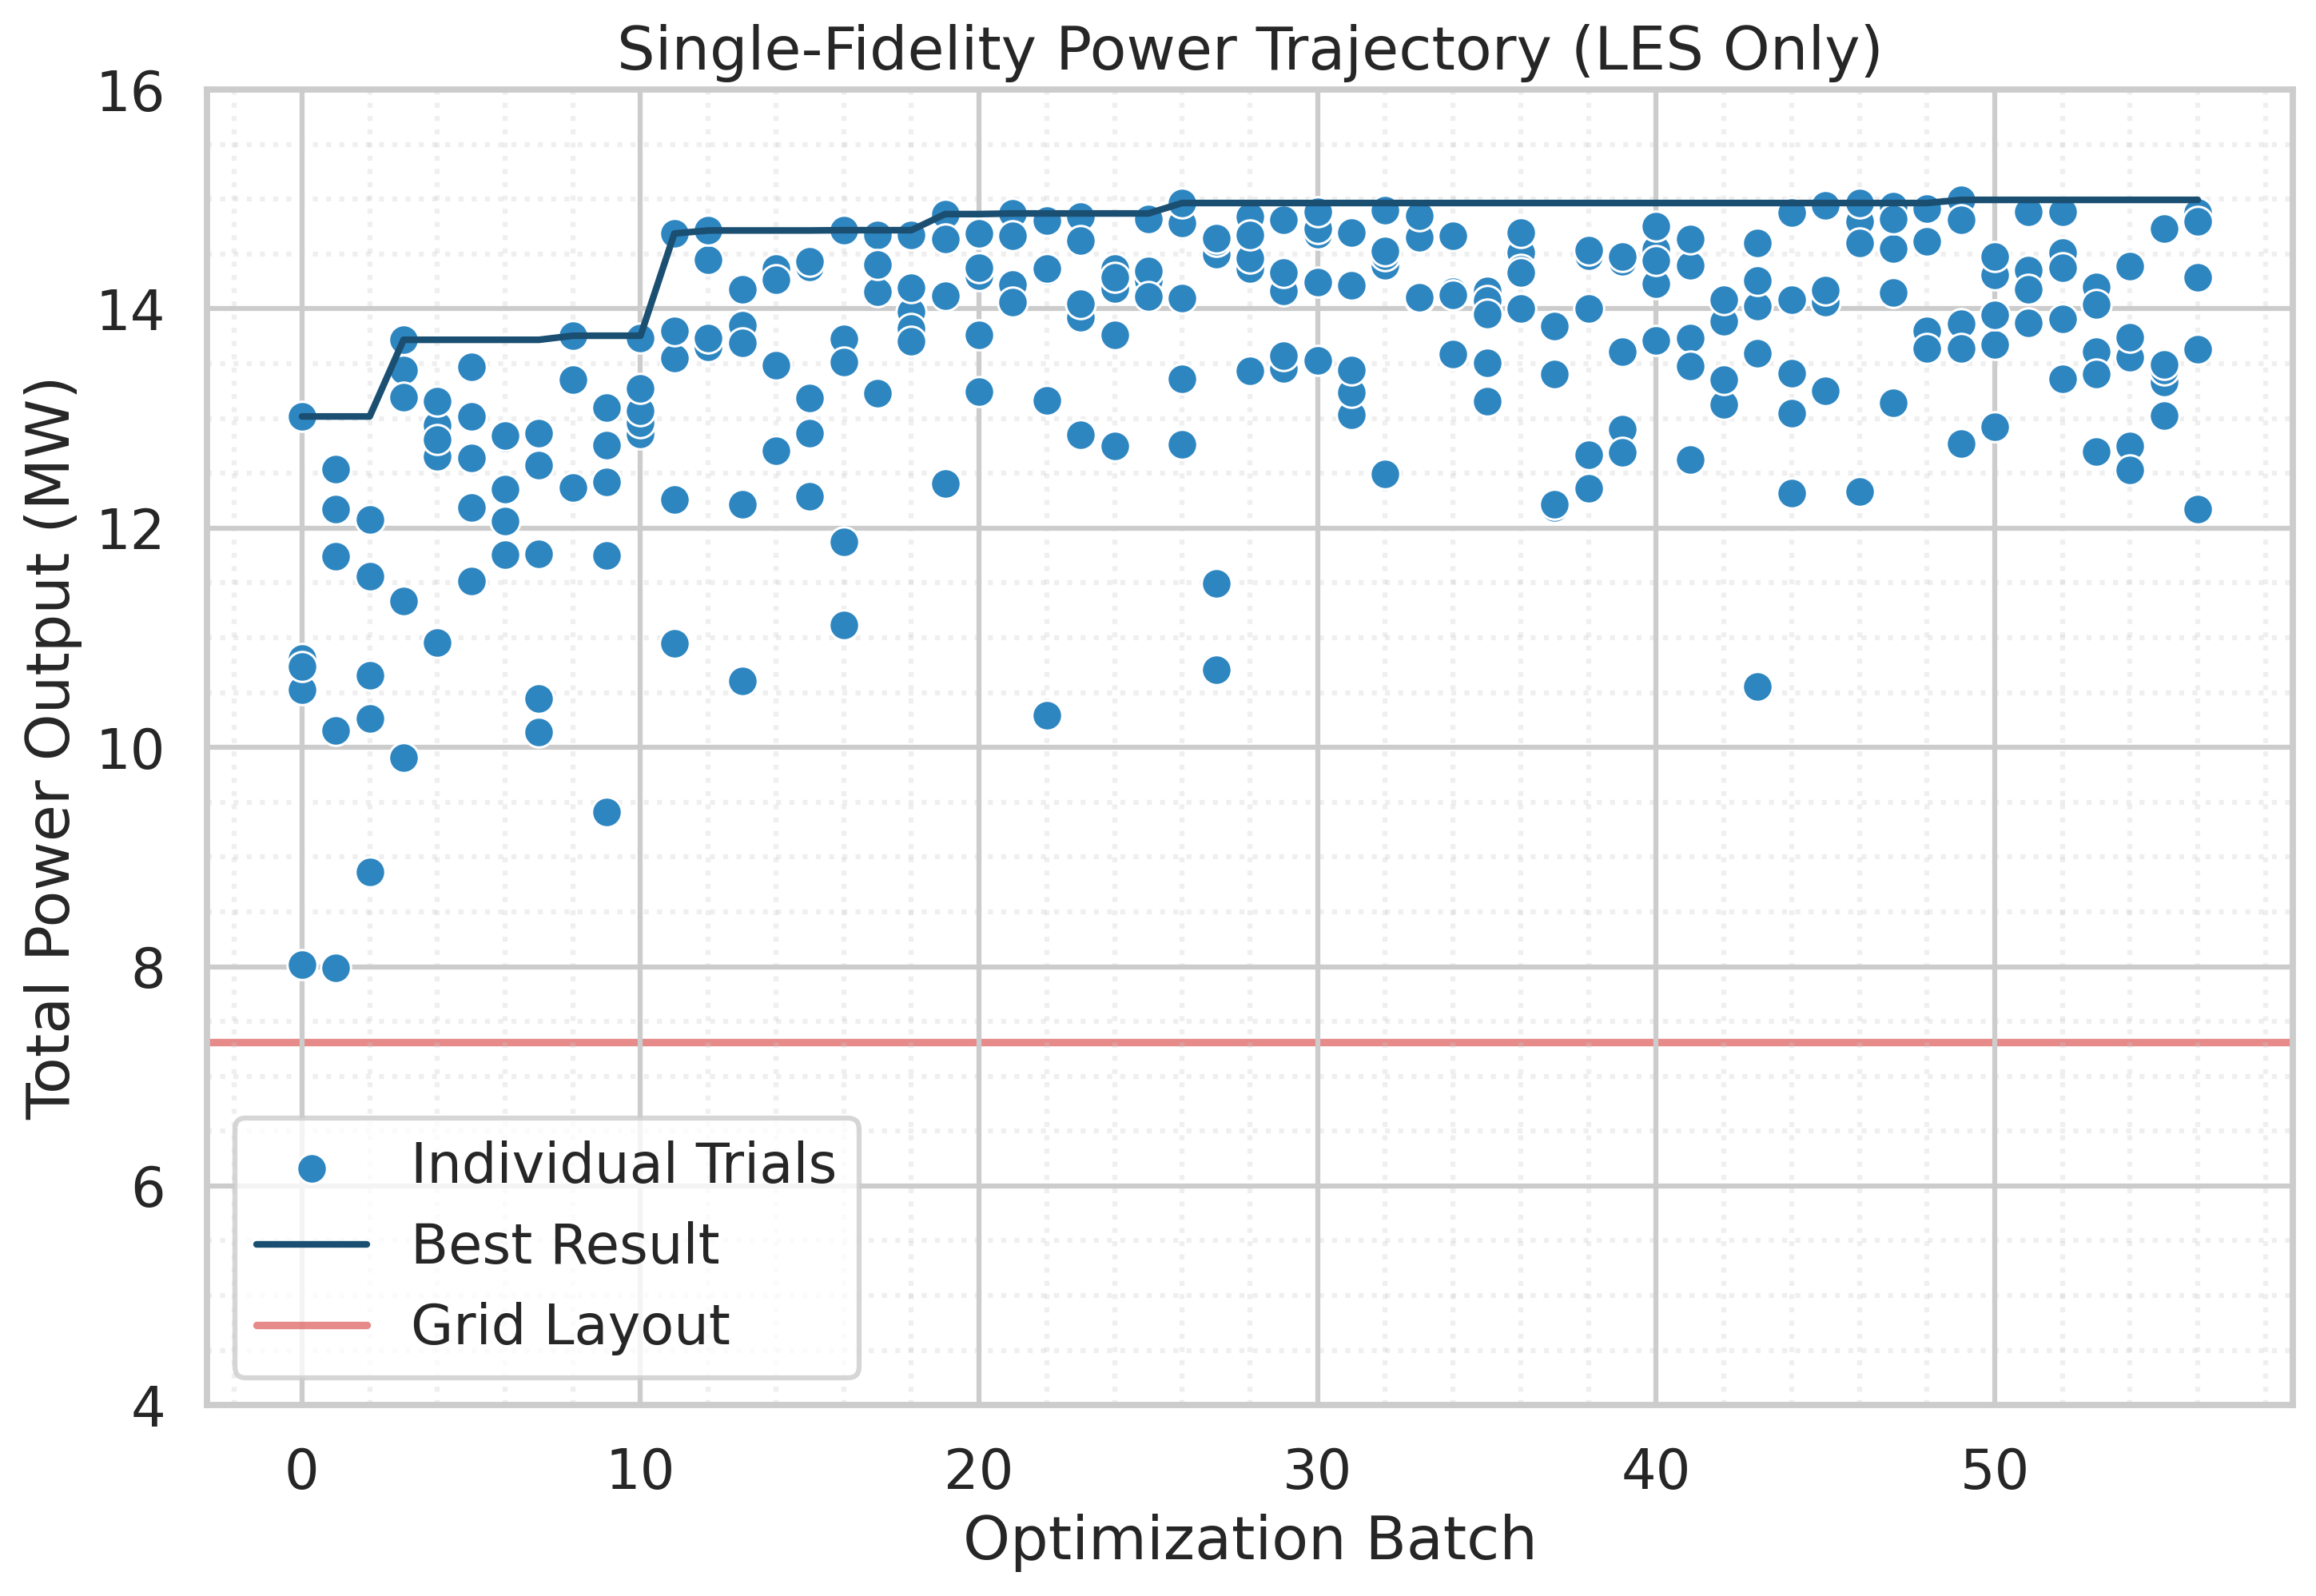
\includegraphics[scale=0.65]{../campaigns/les_only/power_trajectory.png}
    \caption{LES-only Campaign Power Trajectory. Each batch is 5 LES trials.
    }
    \label{fig:les_only_trajectory}
\end{figure}
\begin{figure}[htbp]
    \centering
    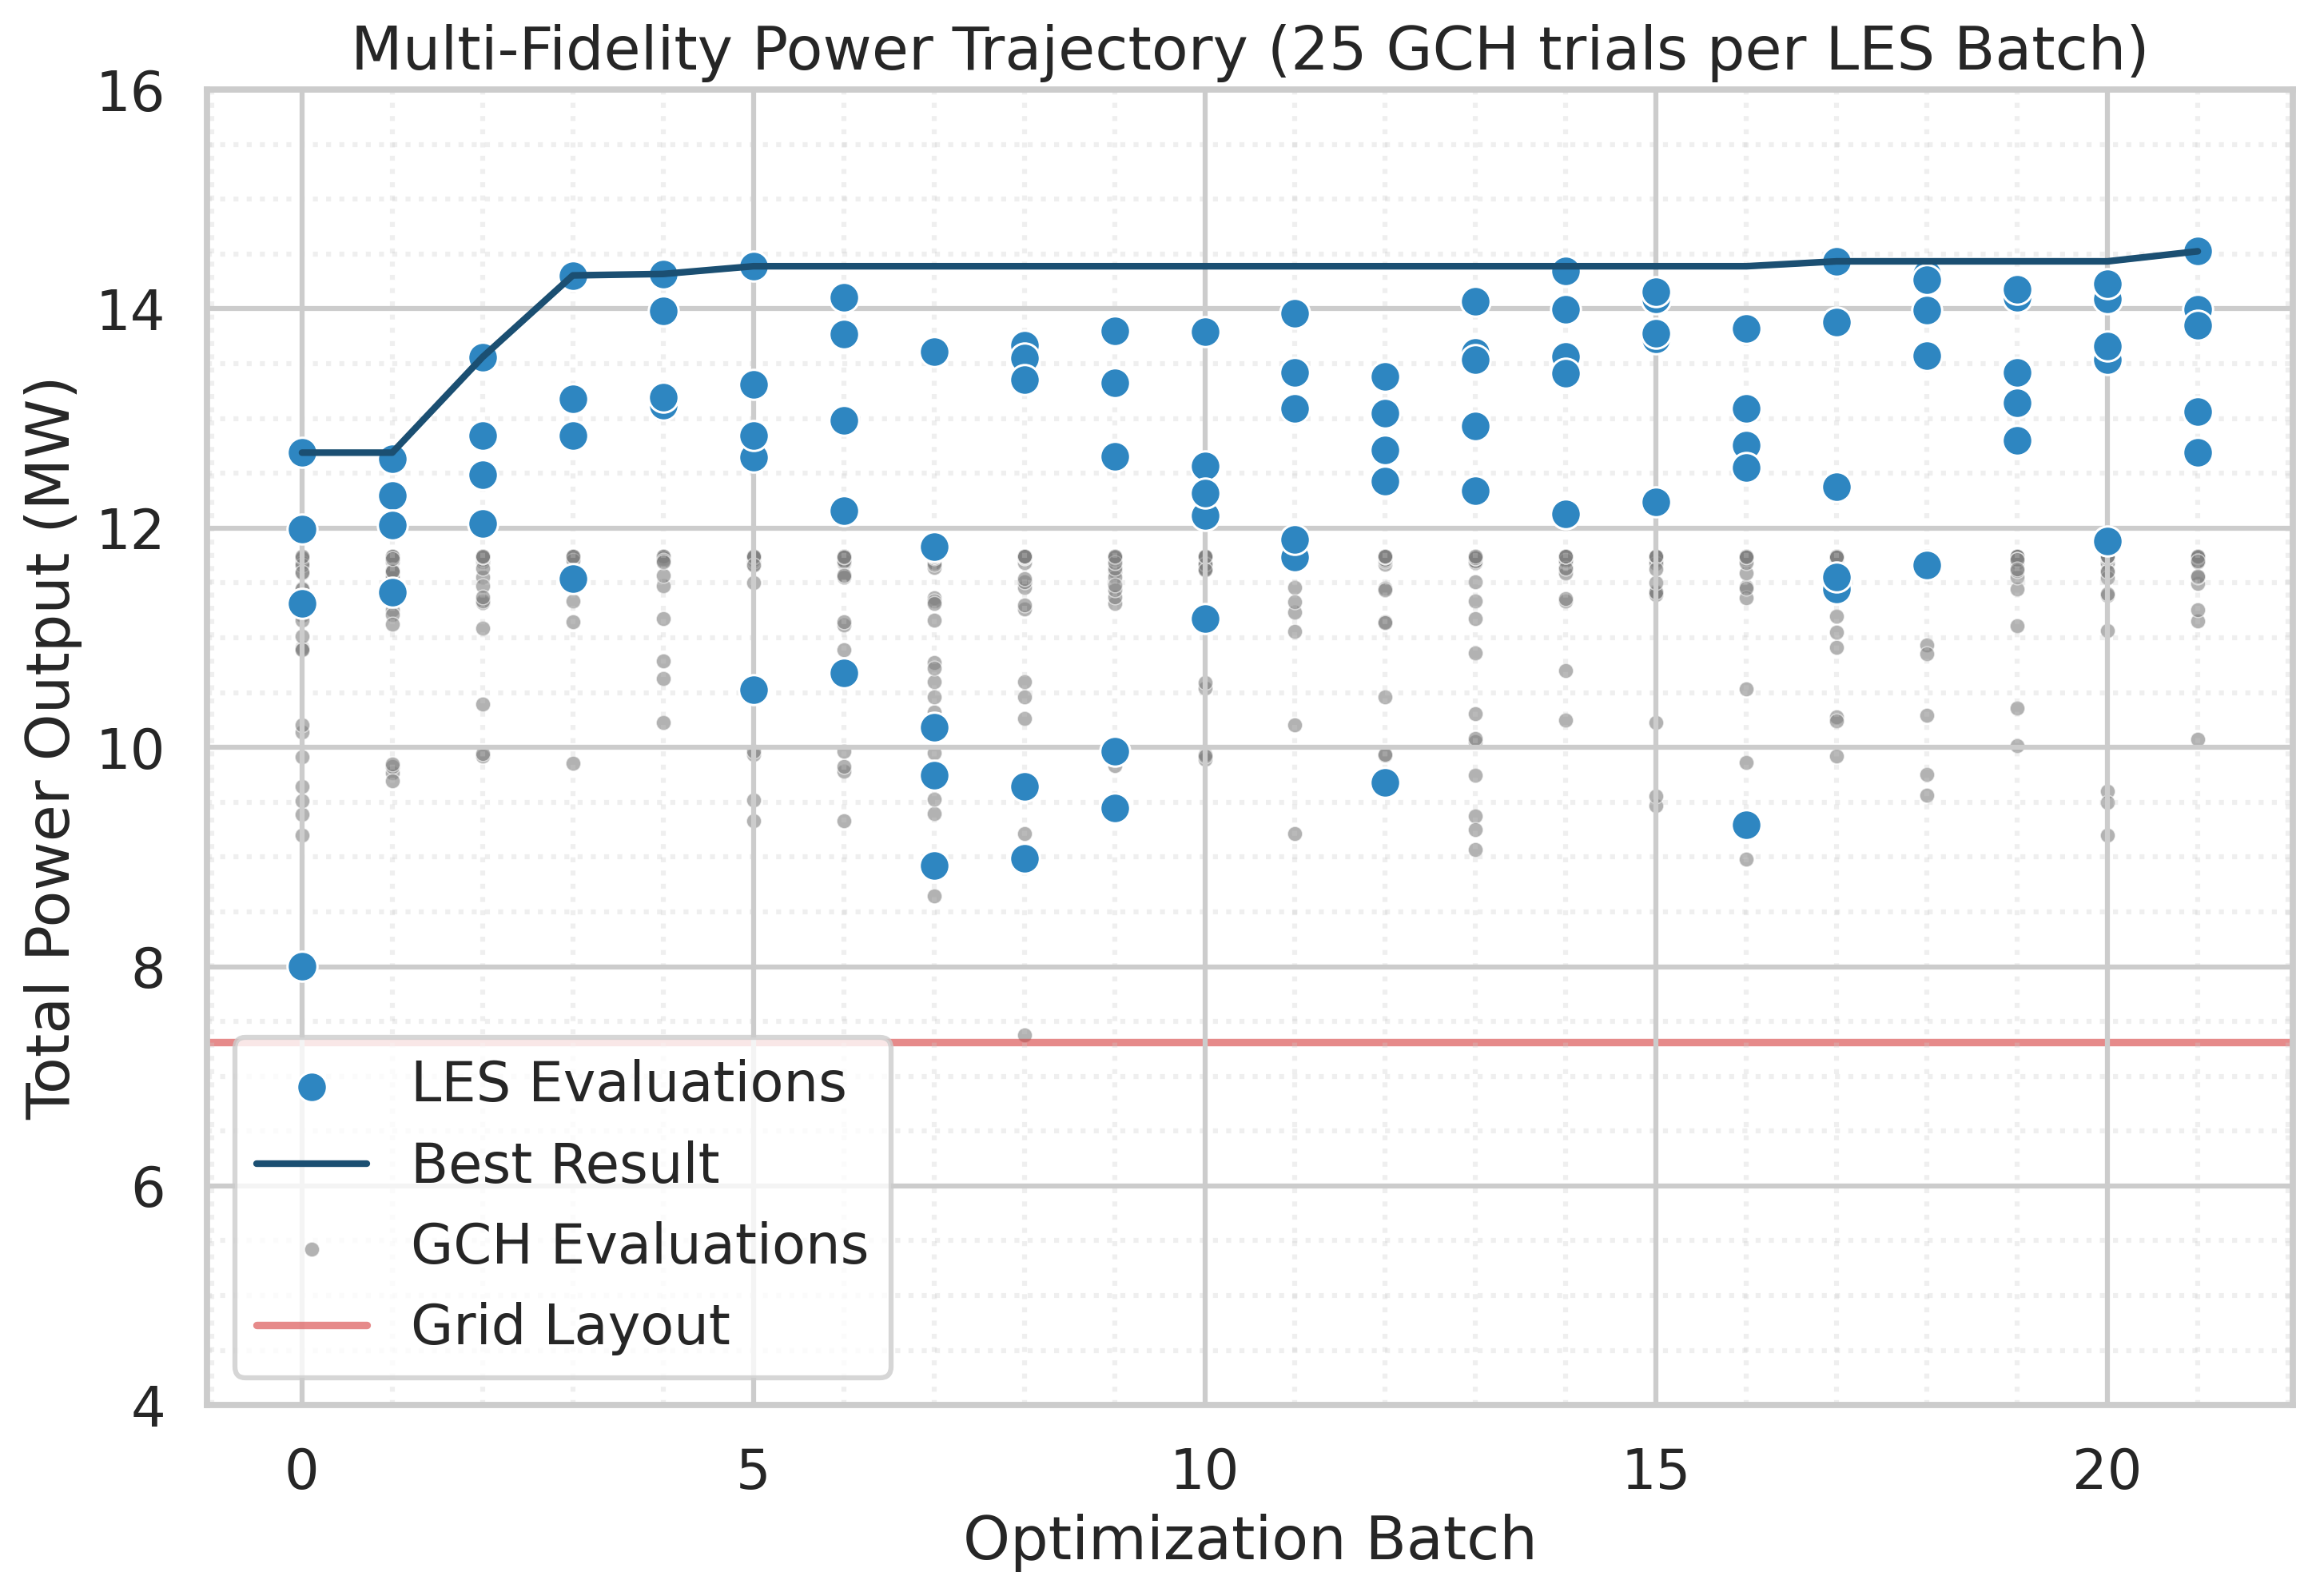
\includegraphics[scale=0.65]{../campaigns/mf_alternating/power_trajectory.png}
    \caption{Multi-fidelity power trajectory. Each "optimization batch" represents
        5 GCH batches of 5 trials each, and one LES batch of 5 trials. GCH evaluations are
        in grey, and LES evaluations are in blue.
    }
    \label{fig:mf_alternating_trajectory}
\end{figure}

The following figures show the instantaneous and mean (over 2 simulated hours)
velocity for the best layouts found by the single fidelity (Figure
\ref{fig:les_only_velocity_flow}) and multi-fidelity campaigns (Figure
\ref{fig:multi_fidelity_flow}).

\clearpage

\begin{figure}[htbp]
    \centering
    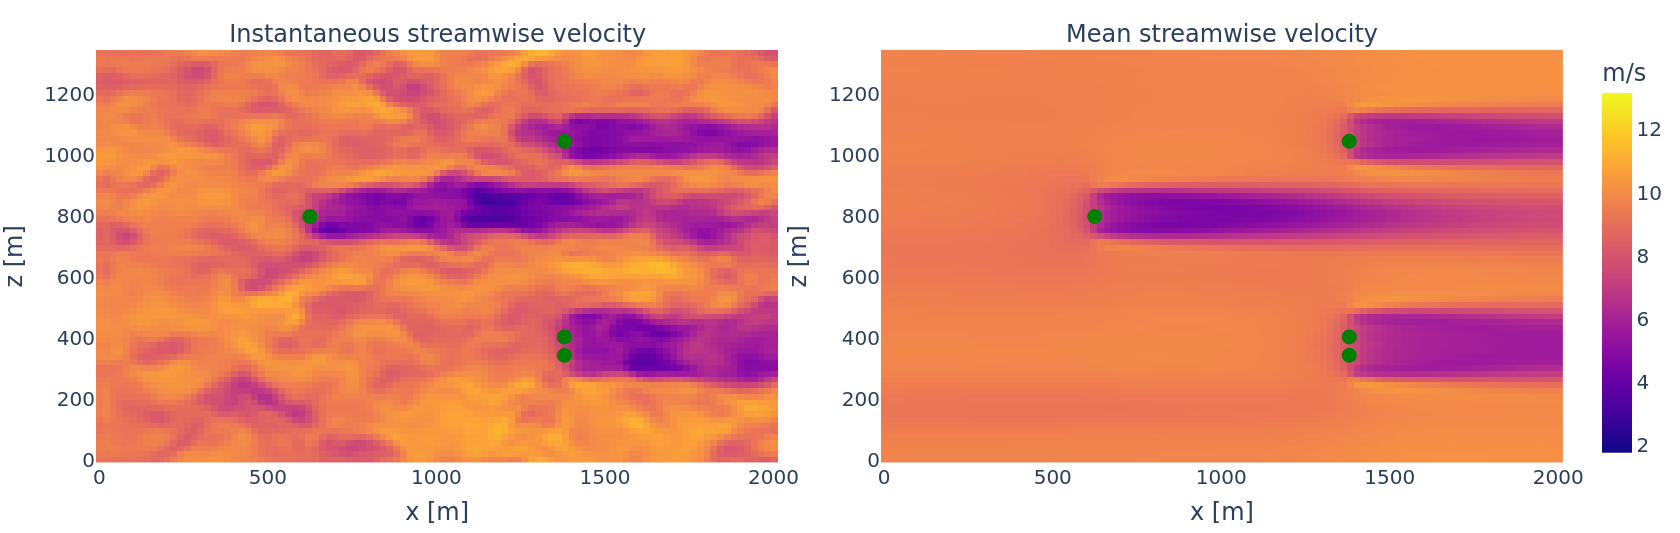
\includegraphics[scale=0.25]{les_only_146.png}
    \caption{Best configuration found by the LES-only campaign. Instantaneous
        snapshot of the velocity flow at 1hr of simulated time past spinup, mean flow
        averaged over a 2hr period.
    }
    \label{fig:les_only_velocity_flow}
\end{figure}

\begin{figure}[htbp]
    \centering
    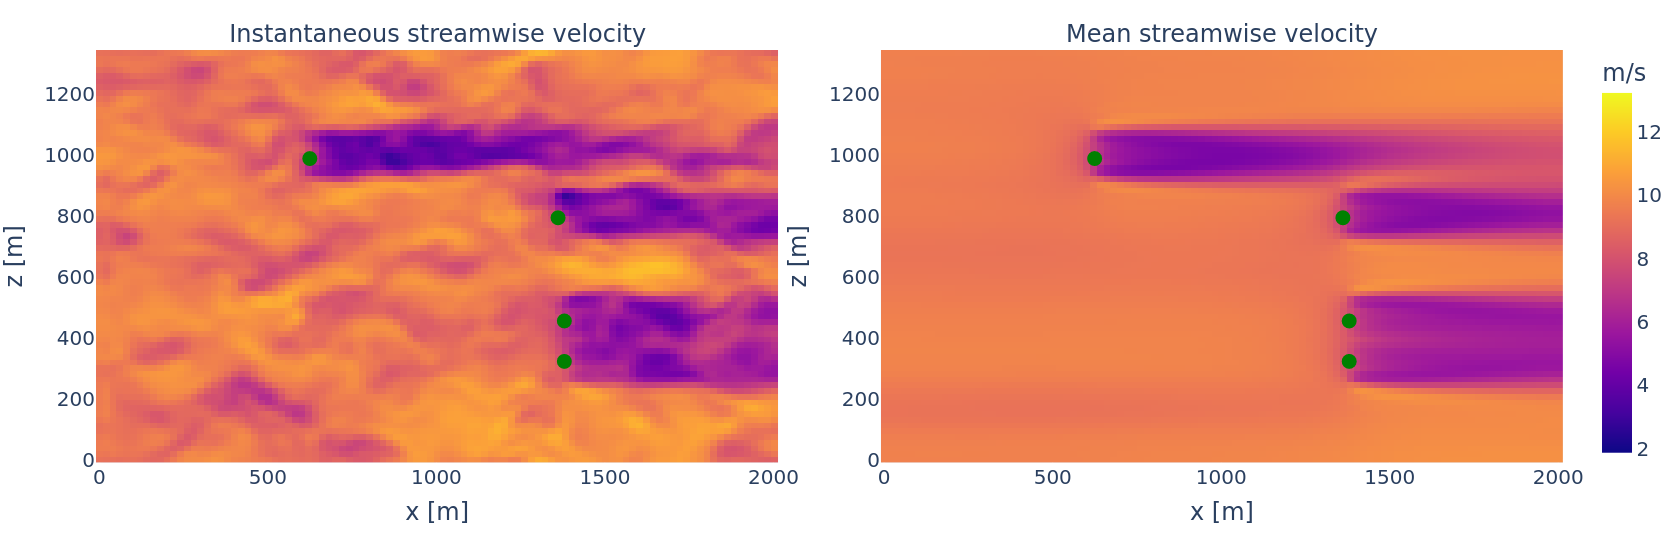
\includegraphics[scale=0.25]{mf_743.png}
    \caption{Best configuration found by the multi-fidelity campaign. Instantaneous
        snapshot of the velocity flow at 1hr of simulated time past spinup, mean flow
        averaged over a 2hr period.
    }
    \label{fig:multi_fidelity_flow}
\end{figure}

\subsection{Fixed BCs}
\label{section:bcs}
Before, a periodic boundary condition was used in the streamwise direction, artificially
adding more turbulence than should occur. I fixed this, and find that it stabilizes
power production throughout the duration of a large-eddy simulation.

Figure \ref{fig:power_convergence} shows the instantaneous and time-averaged
power production of simulations with two different layouts. Figure
\ref{fig:old_power_convergence} shows the same layouts, under the OLD
simulation with incorrect boundary conditions. Compare the left-hand plots in
Figure \ref{fig:old_power_convergence} to those in \ref{fig:power_convergence} (both
use precursor simulations).

This increased stability suggests to me that we can dramatically reduce the
duration for which we run a simulation with limited loss in accuracy of the
time-averaged power output.

\begin{figure}[htbp]
    \centering
    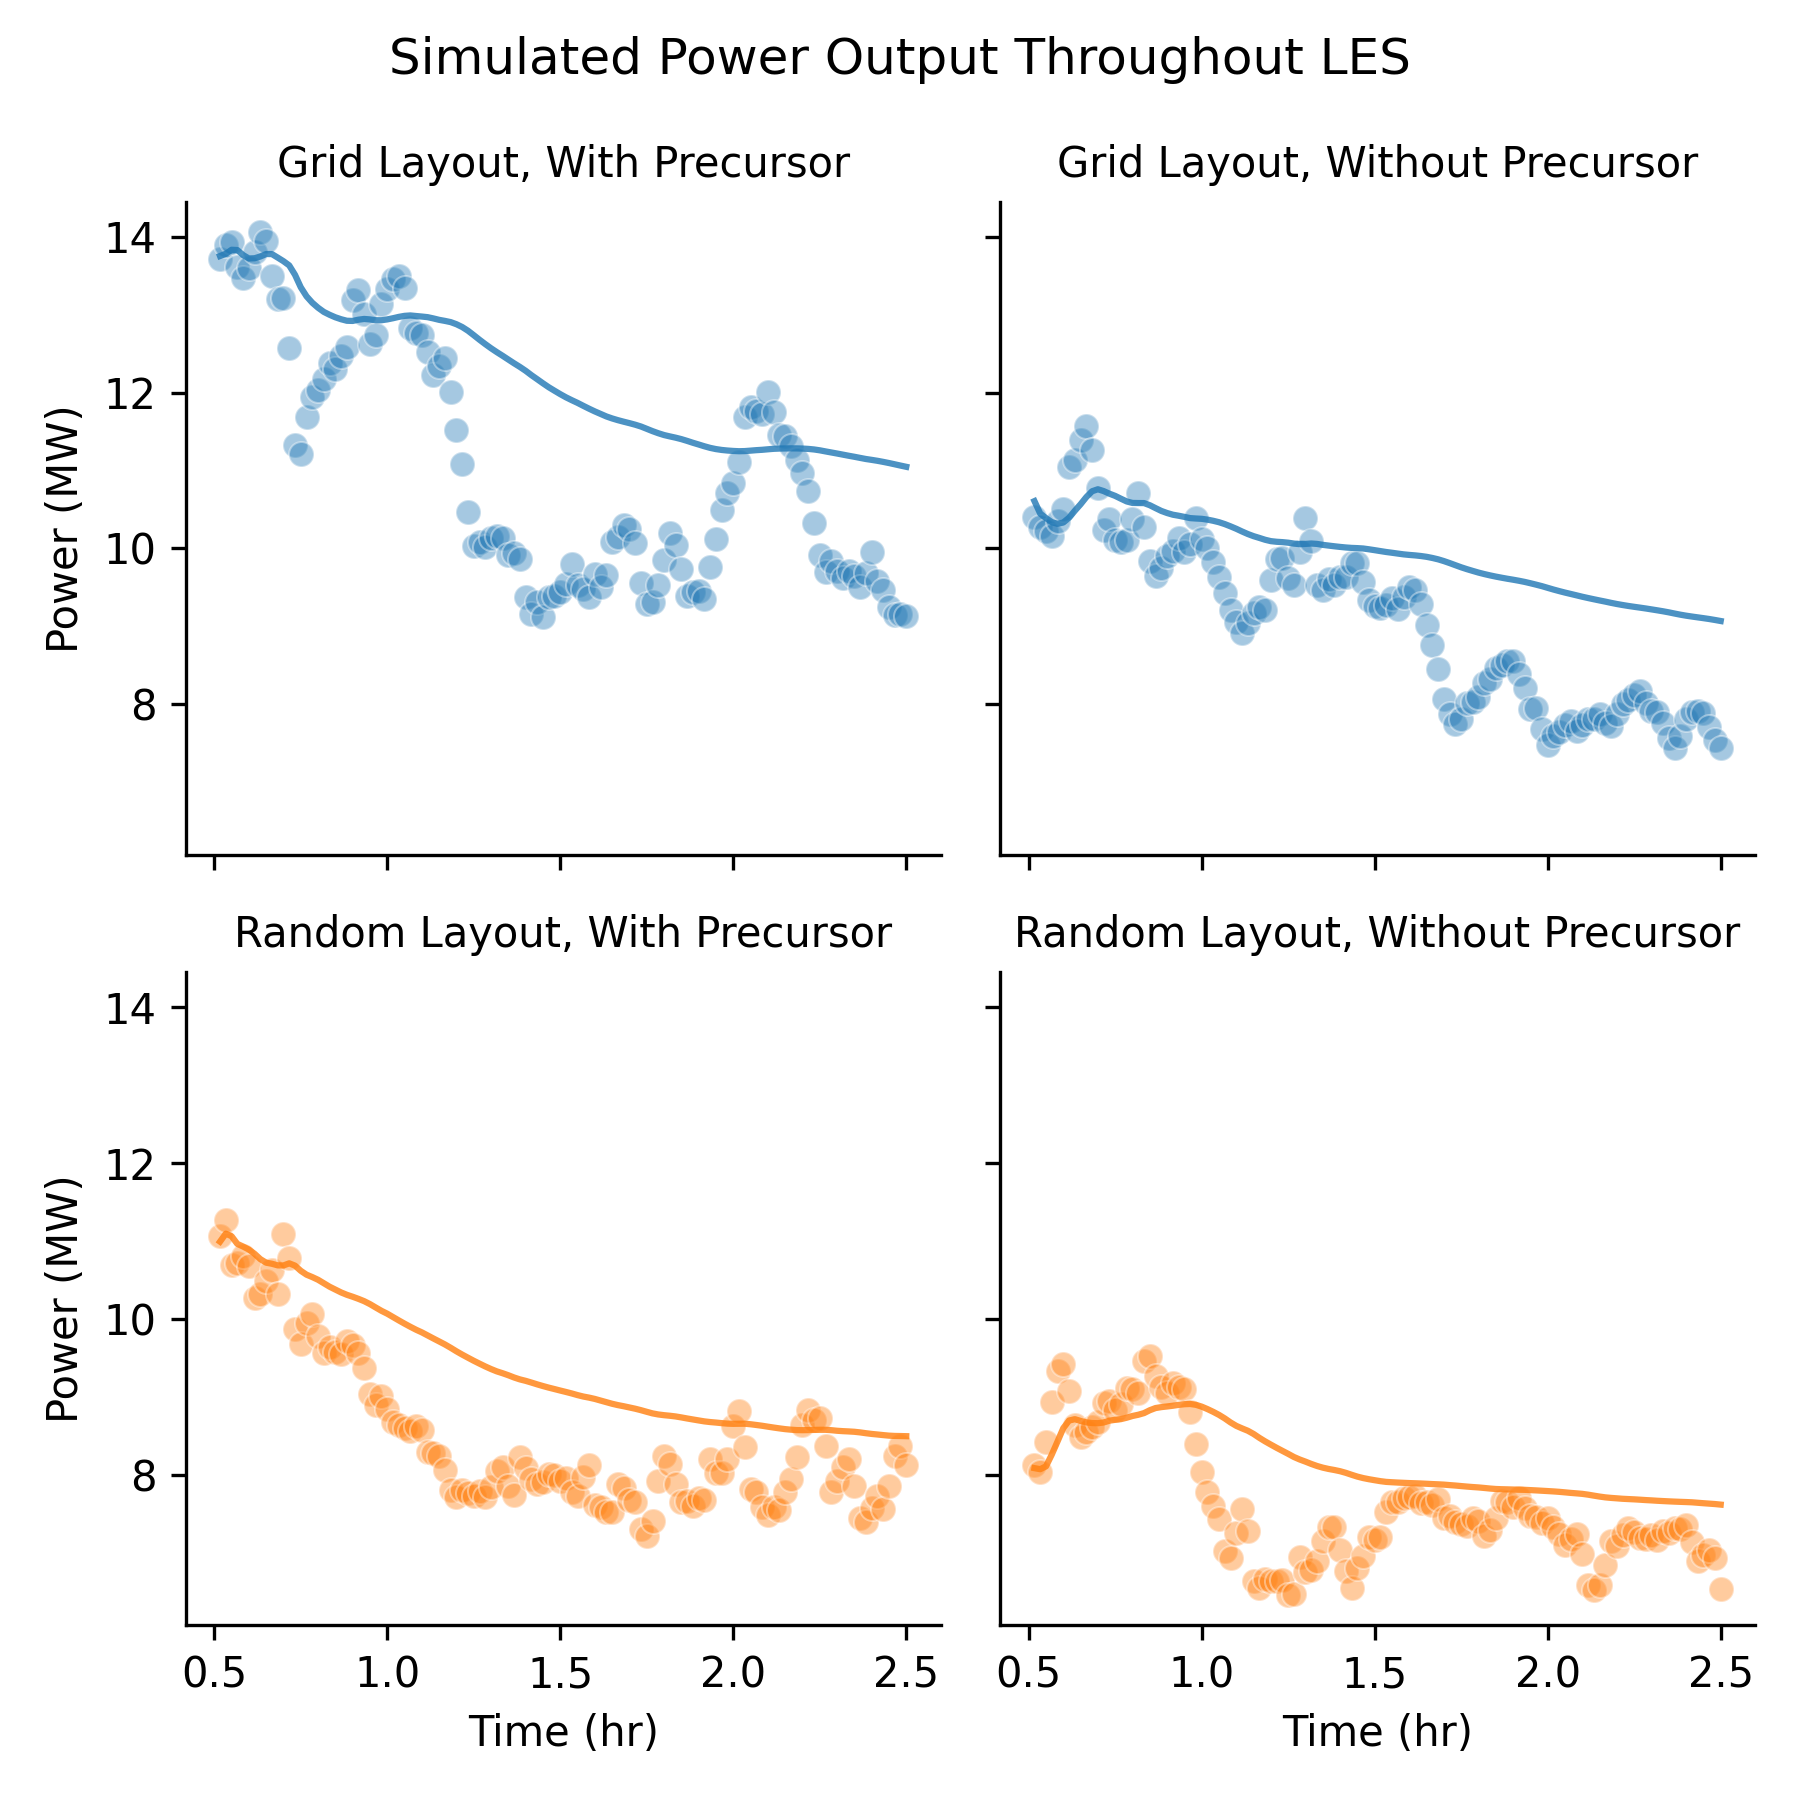
\includegraphics[scale=0.4]{power_convergence.png}
    \caption{Power convergence throughout a large-eddy simulation, for a grid
    layout and a randomly generated turbine layout.}
    \label{fig:power_convergence}
\end{figure}

\begin{figure}[htbp]
    \centering
    \includegraphics[scale=0.7]{old_power_convergence.png}
    \caption{Old power convergence, with INCORRECT boundary conditions, with the same layouts.}
    \label{fig:old_power_convergence}
\end{figure}

\end{document}

%%% Local Variables:
%%% mode: latex
%%% TeX-master: t
%%% End:
% fonts
